\documentclass[a4paper,11pt]{article}

\usepackage{../../Styles/Cours}


\newcommand{\chnum}{Chapitre 16}
\newcommand{\chtitle}{Propagation de la lumière}
\newcommand{\dtype}{TP}

\begin{document}
\maketitle

En se basant sur les documents fournis et des recherches personnelles, proposer une explication des phénomènes observés dans les vidéos 1 et 2, en se reposant sur des schémas.

\section{La plaque de verre}
\begin{table}[h!]
	\begin{tabular}{|>{\centering}m{5cm}|>{\centering}m{5cm}|>{\centering\arraybackslash}m{7cm}|}
	\hline
	Ressource & Observations & Schéma de la situation\\
	\hline
	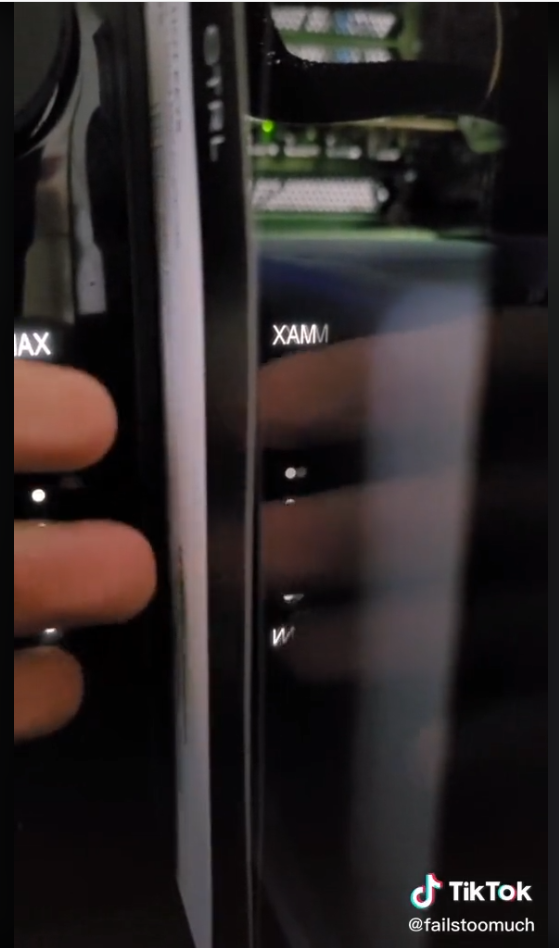
\includegraphics[scale=.3]{Ressources/2GT_C2_Fig1.png}& &\\
	\hline
	\end{tabular}
\end{table}

\section{La pièce}
\begin{table}[h!]
	\begin{tabular}{|>{\centering}m{5cm}|>{\centering}m{5cm}|>{\centering\arraybackslash}m{7cm}|}
	\hline
	Ressource & Observations & Schéma de la situation\\
	\hline
	
\includegraphics[scale=.25]{Ressources/2GT_C2_Fig2.png}& &\\
	\hline
	\end{tabular}
\end{table}

\section{Mise en situation}
Lorsque la lumière passe d'un milieu à un autre, deux phénomènes se mettent en place :
\begin{itemize*}
	\item une partie de la lumière est reflétée par la surface, agissant comme un miroir
	\item une autre partie de la lumière est réfractée : sa direction de propagation change. C'est ce phénomène qui est à l'origine des déformations apparentes que l'on constate lorsque l'on regarde un objet plongé dans l'eau.
\end{itemize*}

\section{Le phénomène de réfraction}
La réfraction vient du fait que la lumière se déplace à une vitesse différente selon le milieu dans lequel il se déplace : dans le vide ou dans l'air, la lumière a une vitesse maximale ( notée $c=3 \cdot 10^{8}~m \cdot s^{-1}$). Dans d'autres milieux on utilise l'indice de réfraction (noté $n_{milieu}$) définit comme le rapport entre la vitesse de la lumière dans le vide et dans un autre milieu (noté $v_{milieu}$).
\begin{eqnarray}
	n_{milieu}=\frac{c}{v_{milieu}} \nonumber
\end{eqnarray}
$n$ n'a pas d'unité et est toujours > 1 car il n'est pas possible de dépasser la valeur de $c$. Une valeur de $n$ grande indique que la lumière est ralentie par le milieu d'une manière importante.

\section{Les lois de Snell-Descartes}
On appelle :
\begin{itemize*}
	\item \textbf{dioptre} : une interface entre les deux milieux transparents
	\item \textbf{rayon incident} : le rayon lumineux arrivant au dioptre
	\item \textbf{normale} : la droite perpendiculaire au dioptre, passant par le point d'incidence
	\item \textbf{angle incident} : noté $i_1$, l'angle formé par le rayon incident et la normale du dioptre
	\item \textbf{angle de réfraction} : noté $i_2$, l'angle formé par le rayon réfracté et la normale du dioptre
	\item \textbf{angle de réflexion} : noté $r$, l'angle formé apr le rayon réfléchi et la normale
\end{itemize*}

Les lois de Snell-Descartes ont été établies indépendamment par Willebrord Snell et René Descartes au XVIIe siècle :
\begin{itemize}
	\item \textbf{$1^{ère}$ loi de Snell-Descartes} : le rayon incident, le rayon réfracté, le rayon réfléchi et la normale sont dans le même plan.
	\item \textbf{$2^{ème}$ loi de Snell-Descartes} :\\
	Pour la réfraction : 
	\begin{eqnarray}
		n_1 \cdot sin(i_1) = n_2 \cdot sin(i_2) \nonumber 
	\end{eqnarray}
	Pour la reflexion :
	\begin{eqnarray}
		i_1 = r \nonumber 
	\end{eqnarray}
	avec $n_1$ et $n_2$ respectivement les indices de réfractions des milieux $1$ et $2$.
\end{itemize}
\textbf{Schéma de la situation :}\\
\begin{center}
	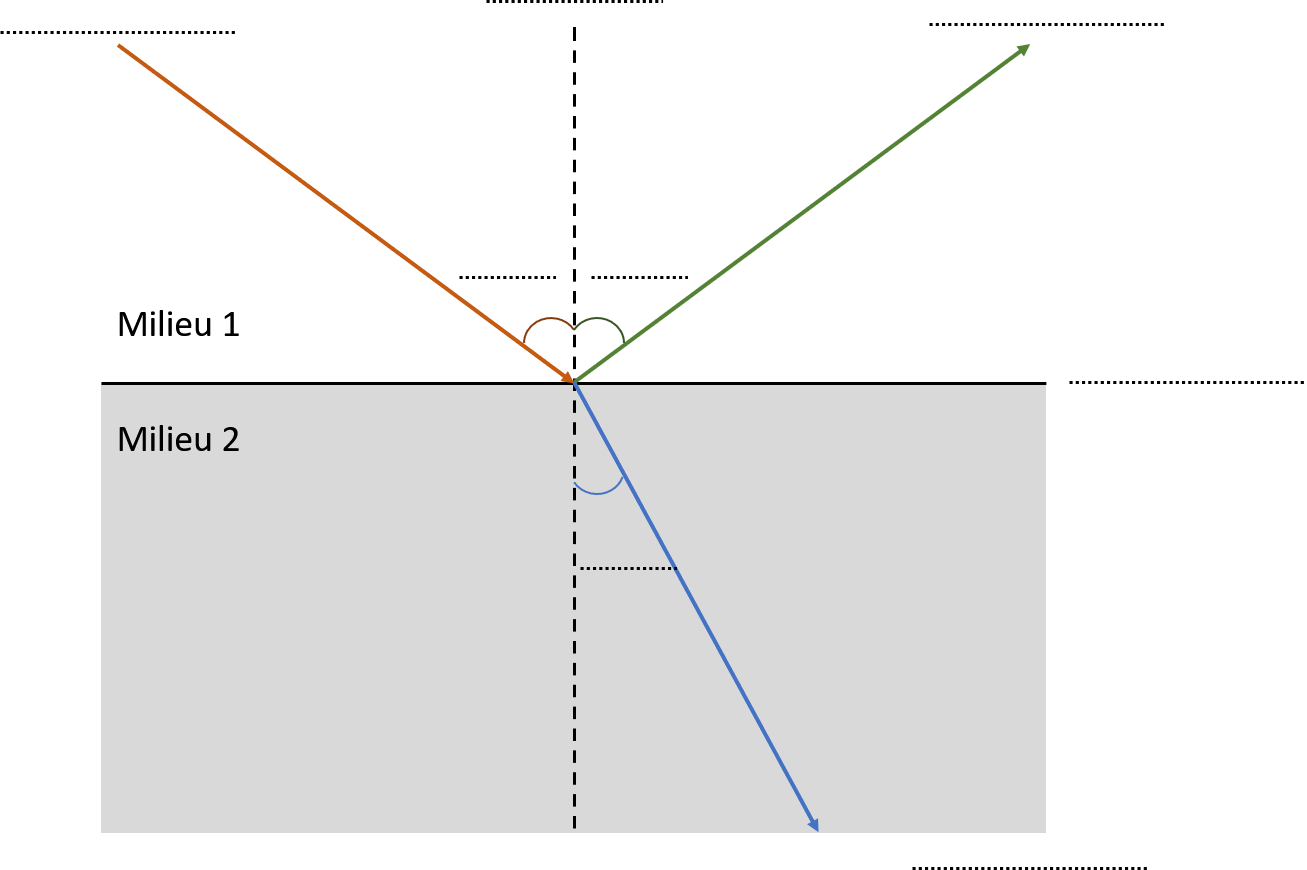
\includegraphics[scale=.6]{Ressources/2GT_C2_Fig3.png}
\end{center}
\end{document}
